\documentclass[letterpaper,12pt]{article}
\usepackage[utf8]{inputenc}

% Format table
\usepackage{booktabs}

% For images
\usepackage{graphicx}
\graphicspath{ {./images/} }

\usepackage{longtable}
\usepackage[backend=biber,style=alphabetic,style=apa]{biblatex}

\addbibresource{mybibliography.bib}

\title{Choosing cities to start a business in Central America}
\author{Luis Diego Quirós}
\date{August, 2021}

\begin{document}

\maketitle

\section{Introduction}

The economic activity in Central America for the last 15 years has been growing more than in the rest of Latin America (\cite{cadena_strengthening_2019}). It is usual for investors to be looking for opportunities to invest in the region. Still, they are faced with tough decisions about the best cities to invest in and the kind of business. Cultural and economic differences between countries and cities can be abysmal, so it is essential to identify coincidences or similarities. Once similar characteristics are recognized, investing will be more attractive because long-term expansion plans can be designed.

Understanding consumption patterns and trends is complex due to the limited or deficient information found in government pages about economic sectors in the region. Identifying actual thriving venues categories is very beneficial as an insight into industries that have grown or are still needed to complement existing ones. This information is helpful to investors or people looking to create new businesses at a regional level in Central America. It will provide them with information to make data-driven decisions. Also, the results can be used to develop commercial plans based on the reality of each country or cluster of cities giving more certainty about the probabilities for the business to survive.

\section{Data acquisition and cleaning}

The needed information is 1) the most important cities in each country of Central America and 2) trending venues in each city. Multiple sources are considered to gather the data required for the project.

\subsection{Data sources}

\textbf{Wikipedia}

Wikipedia was used to get the most significant cities of each country. The most populous cities of each country are going to be chosen. The information obtained from here will be the country and the name of the city.

\textbf{Nominatim}

Nominati is a tool used for geocoding. Based on the country and name of the city, it generated the corresponding latitude and longitude. 

\textbf{Foursquare}

Foursquare was used to get information about the trending venues and their category

\section{Methodology}

The following process will be followed:

\subsection{Identify important cities}

The most prominent cities were scraped using the corresponding Wikipedia page for each country, gathering their name and province. Beautiful Soup was the python package used for scraping (\cite{richardson2007beautiful}). The obtained cities are identified in Table \ref{tab:table1}. The latitude and longitude of each city were obtained through geocoding. The geographical information is essential to reference and identify venues around the corresponding points.

\subsection{Identify trending venues categories}

Using the Foursquare API for each city, trending venues were obtained. The top 10 locations were selected with a radius of 3 kilometers around the coordinates of the city. The category of each place was gathered from the API as well. 

\subsection{Cluster cities with similar categories}

The data was summarized, so the number of venues in each category was obtained per city. The algorithm used for clustering was k-means with euclidean distance. The number of clusters was selected using inertia and the average of the silhouette coefficients. These metrics were plotted as a function of the number of groups to observe how many were needed.

\section{Results}

A total of 63 cities were chosen (Figure \ref{fig:cities}), and in them, the information of 2,625 venues was obtained. These were divided into 247 categories. The Pizza Places, Restaurant, and Fast Food restaurants were the most abundant kinds (Figure \ref{fig:categories}).

\begin{figure}[h]
    \centering
    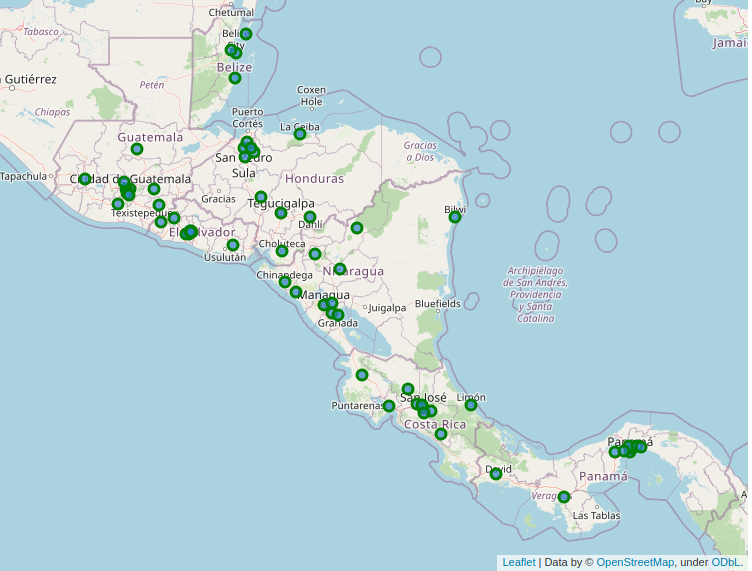
\includegraphics[width=\textwidth]{cities.png}
    \caption{Top 10 venue categories}
    \label{fig:cities}
\end{figure}

\begin{figure}[h]
    \centering
    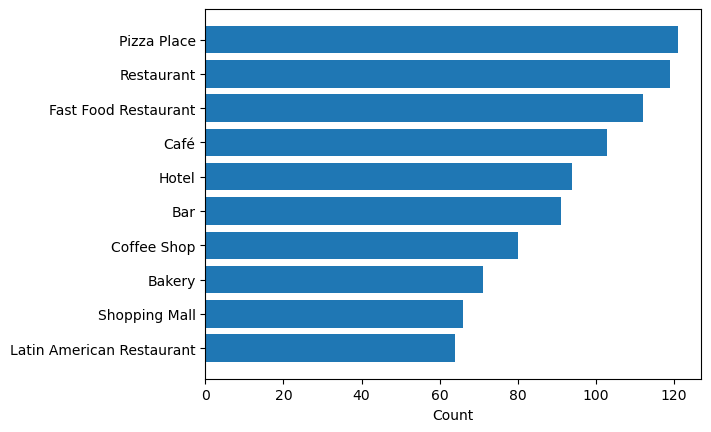
\includegraphics[width=\textwidth]{images/categories.png}
    \caption{Chosen cities across Central America}
    \label{fig:categories}
\end{figure}

The elbow method was used to determine the number of clusters (Figure \ref{fig:metrics}). It was observed that six groups maximize the average silhouette coefficients, and the inertia stopped decreasing considerably \ref{tab:my-table}).

\begin{figure}[h]
    \centering
    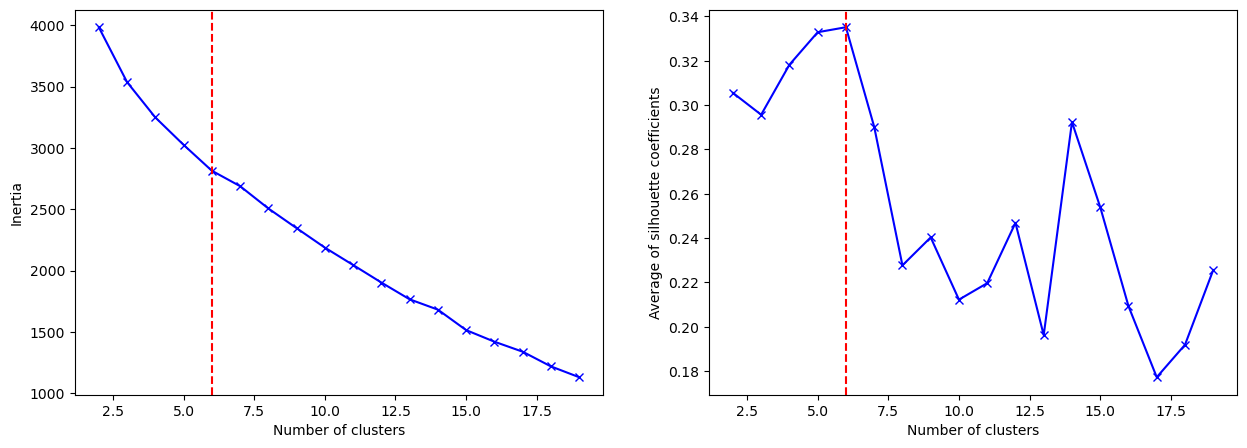
\includegraphics[width=\textwidth]{images/metrics.png}
    \caption{Elbow method to choose the number of clusters}
    \label{fig:metrics}
\end{figure}

\begin{table}[]
\centering
\caption{Cluster sizes}
\label{tab:my-table}
\begin{tabular}{@{}ll@{}}
\toprule
Cluster Numer & Cities \\ \midrule
0             & 26     \\
1             & 11      \\
2             & 8      \\
3             & 5      \\
4             & 5      \\
5             & 3      \\ \bottomrule
\end{tabular}
\end{table}


\subsection{Few businesses cluster}

It is the more significant cluster with 26 cities.  These cities are characterized by having very few businesses (maximum 6), and they are not very diverse because the trending venues are only in the categories Fast Food Restaurant, Hotel and Shopping mall (Figure \ref{fig:cluster_1}). On average, each city has 11 venues.

\begin{figure}[h]
    \centering
    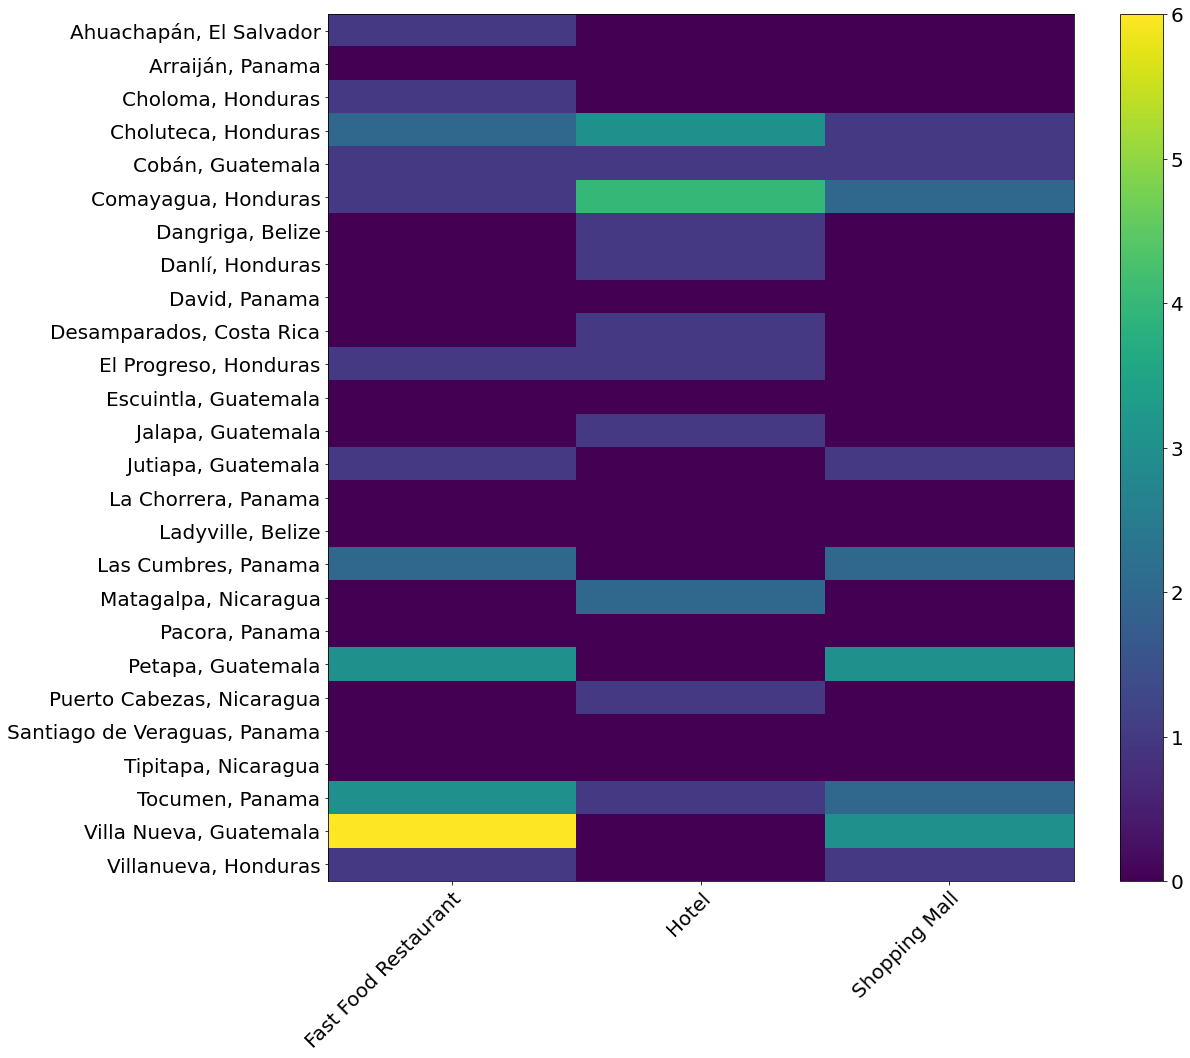
\includegraphics[width=\textwidth]{images/cluster1.png}
    \caption{Number of venues per category on the cities in the few business cluster}
    \label{fig:cluster_1}
\end{figure}

\subsection{Gastronomic cluster}

The cities have, on average, 44 venues. Looking at the distribution of the categories, the most popular are bars,  restaurants, ice cream shops, and fast-food restaurants (Figure \ref{fig:cluster_2}). All of them are related to food which is where the cluster name derives. 

\begin{figure}[h]
    \centering
    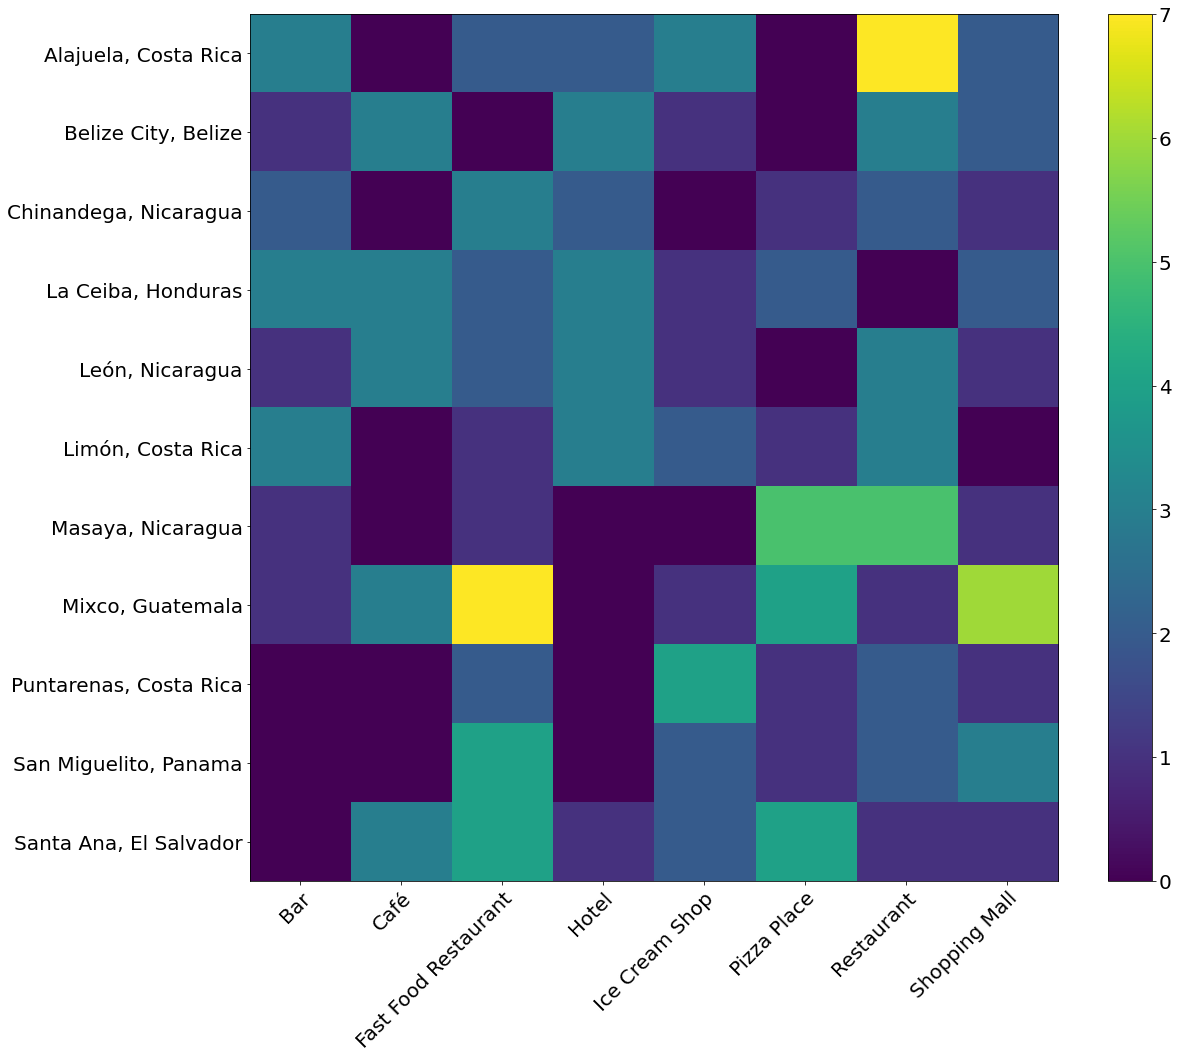
\includegraphics[width=\textwidth]{images/cluster2.png}
    \caption{Number of venues per category on the cities in the gastronomic cluster}
    \label{fig:cluster_2}
\end{figure}


\subsection{Busy Cluster}

It is the cluster with the highest amount of venues per city. On average, each city has 95. The categories with the most revenues are similar to the gastronomic group, but the density is higher. Also, the most abundant venues are bakeries, coffee shops, and steak houses (Figure \ref{fig:cluster_3})

\begin{figure}[h]
    \centering
    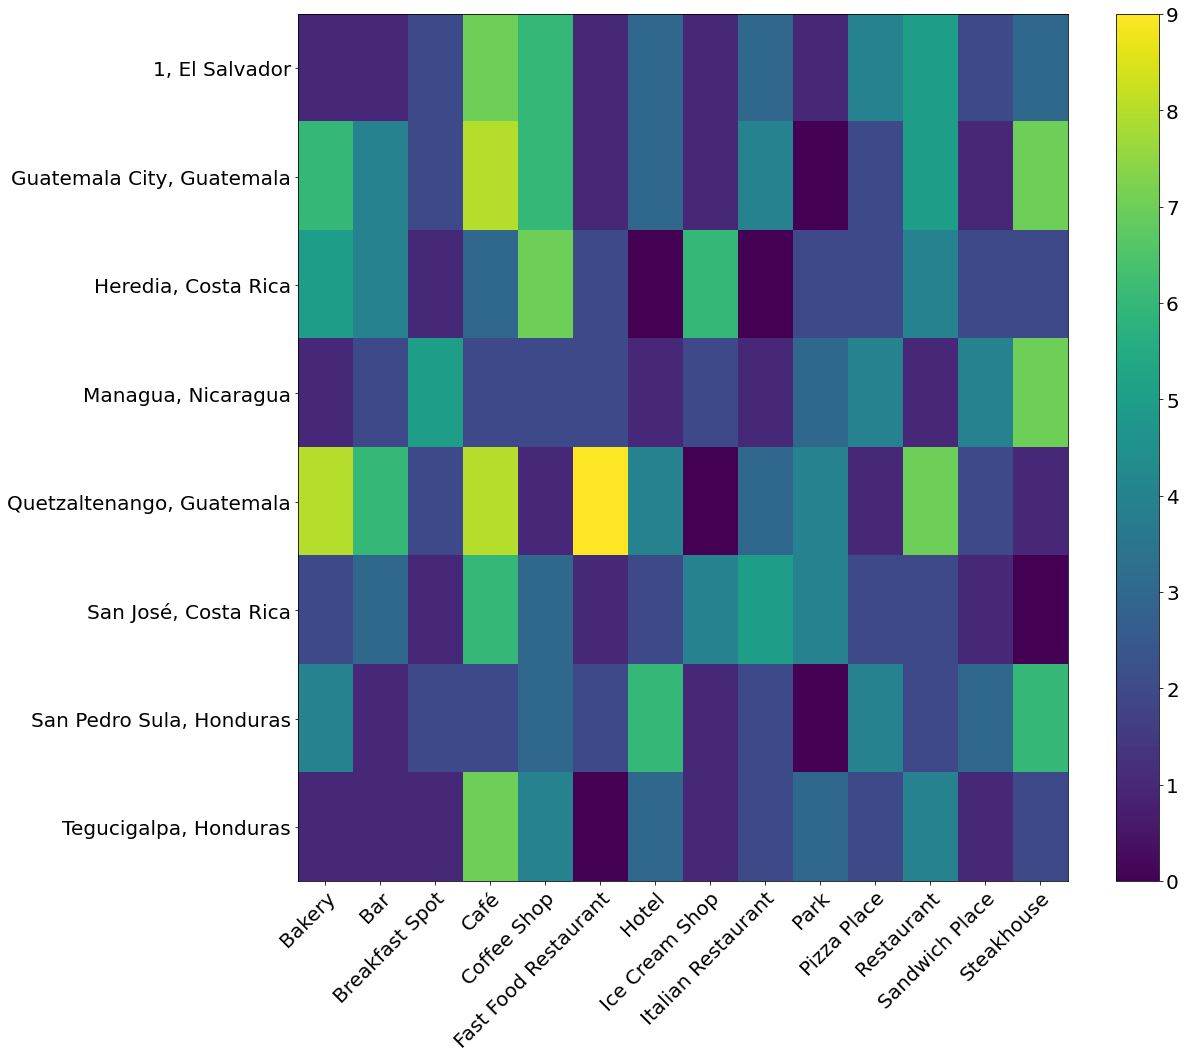
\includegraphics[width=\textwidth]{images/cluster3.png}
    \caption{Number of venues per category on the cities in the busy cluster}
    \label{fig:cluster_3}
\end{figure}


\subsection{Smaller Clusters}

The other clusters are tiny, but the cities have a very high number of venues. Cluster 3 is mainly formed by cities of Costa Rica, and on average, they have 85 venues. (Figure \ref{fig:cluster_3}). Cluster 4 has only cities from El Salvador. It has five cities, and on average, each one has 88 venues. (Figure \ref{fig:cluster_4}). Cluster 5 is the smallest one with only three cities, and on average, they have 69 venues. They are characterized because the most relevant venues are in the categories of hotels and restaurants. This is setting the cities apart because Granada, Nicaragua, has the most trending hotels (Figure \ref{fig:cluster_5}).

\begin{figure}[h]
    \centering
    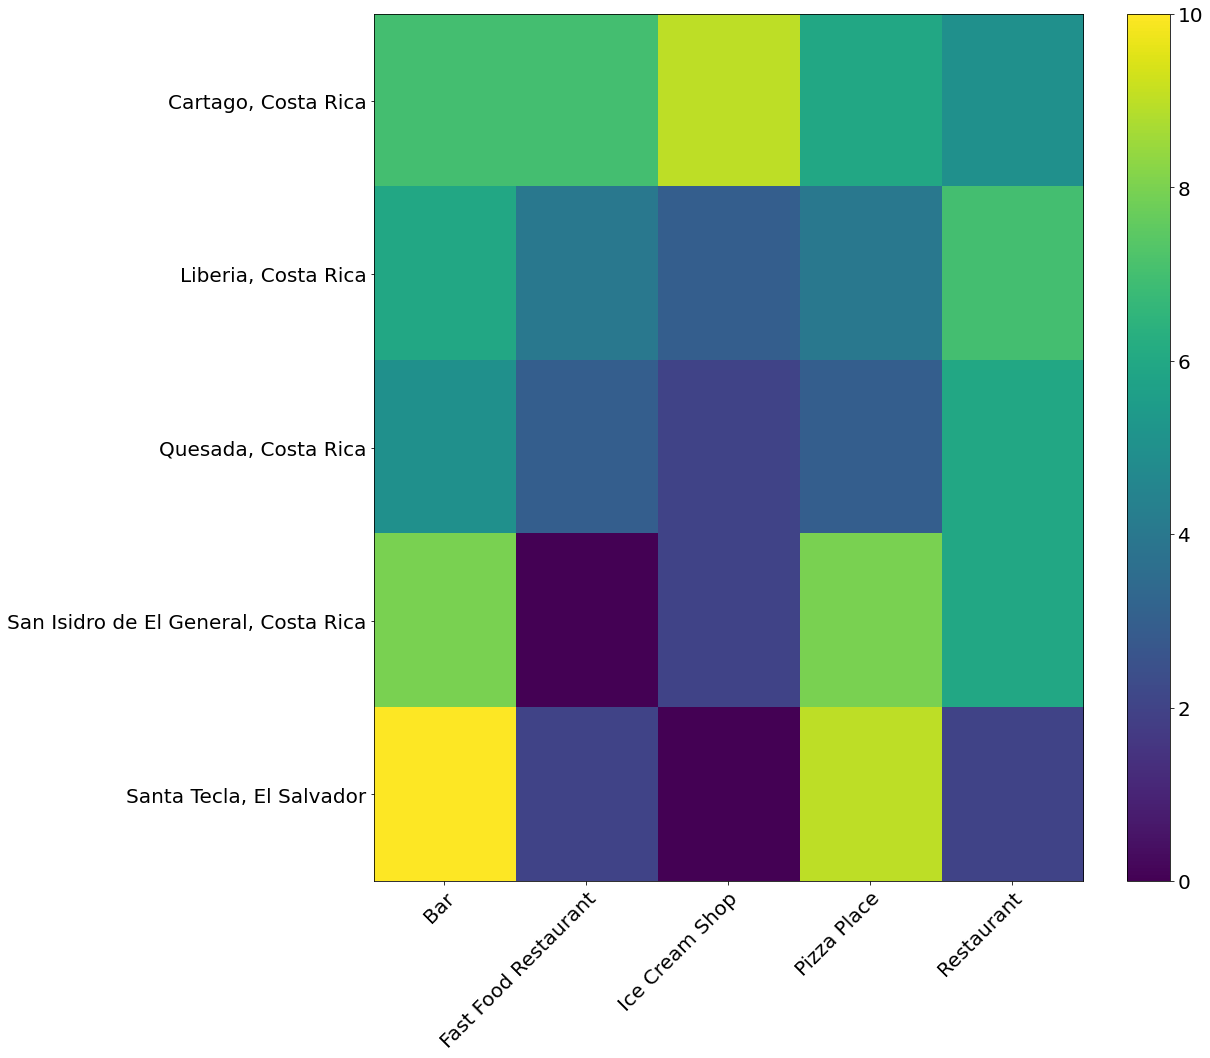
\includegraphics[width=\textwidth]{images/cluster4.png}
    \caption{Number of venues per category on the cities in the small cluster 1}
    \label{fig:cluster_3}
\end{figure}

\begin{figure}[h]
    \centering
    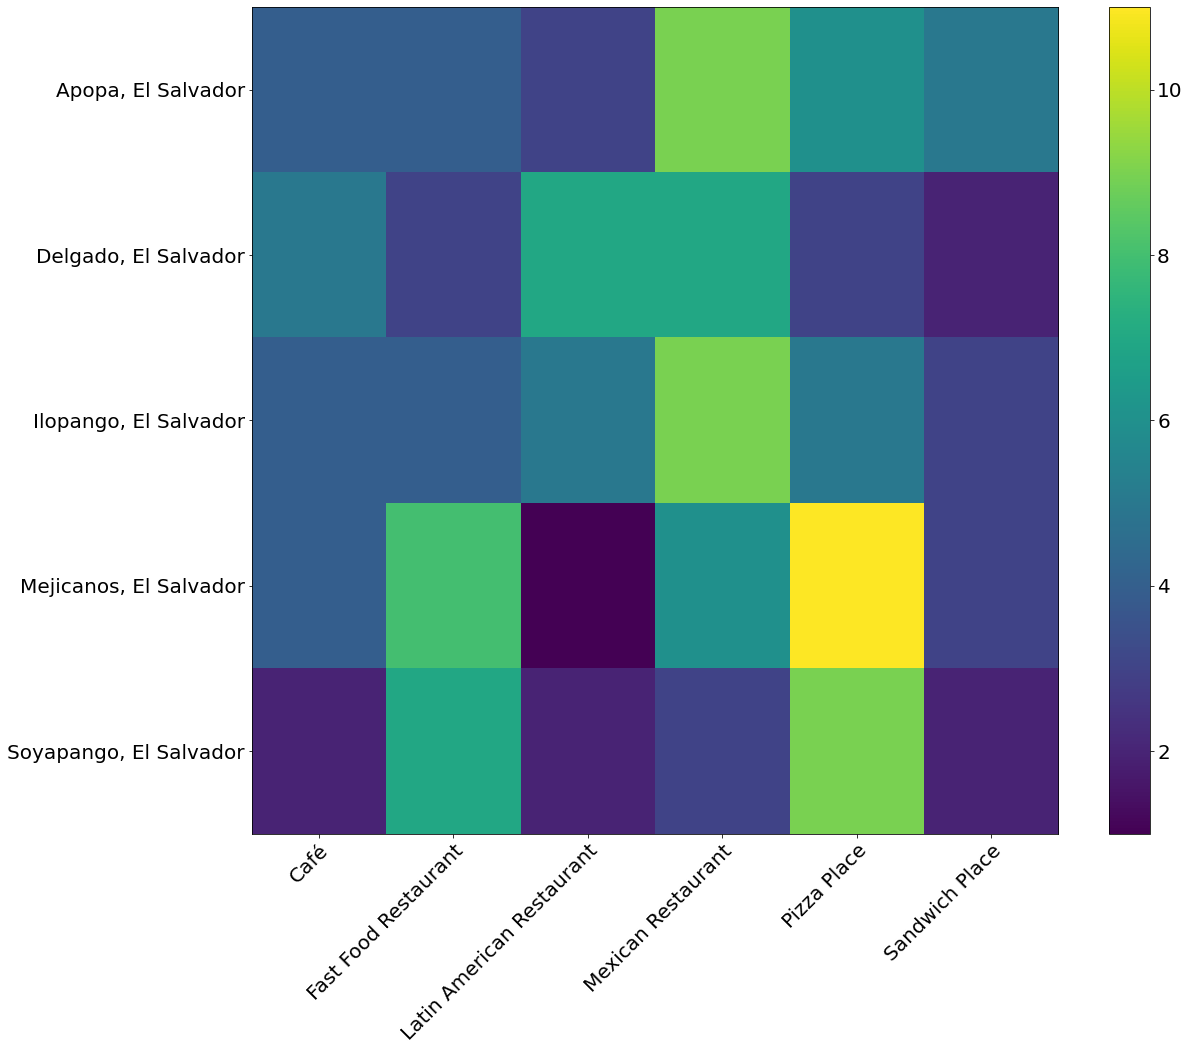
\includegraphics[width=\textwidth]{images/cluster5.png}
    \caption{Number of venues per category on the cities in the small cluster 2}
    \label{fig:cluster_4}
\end{figure}


\begin{figure}[h]
    \centering
    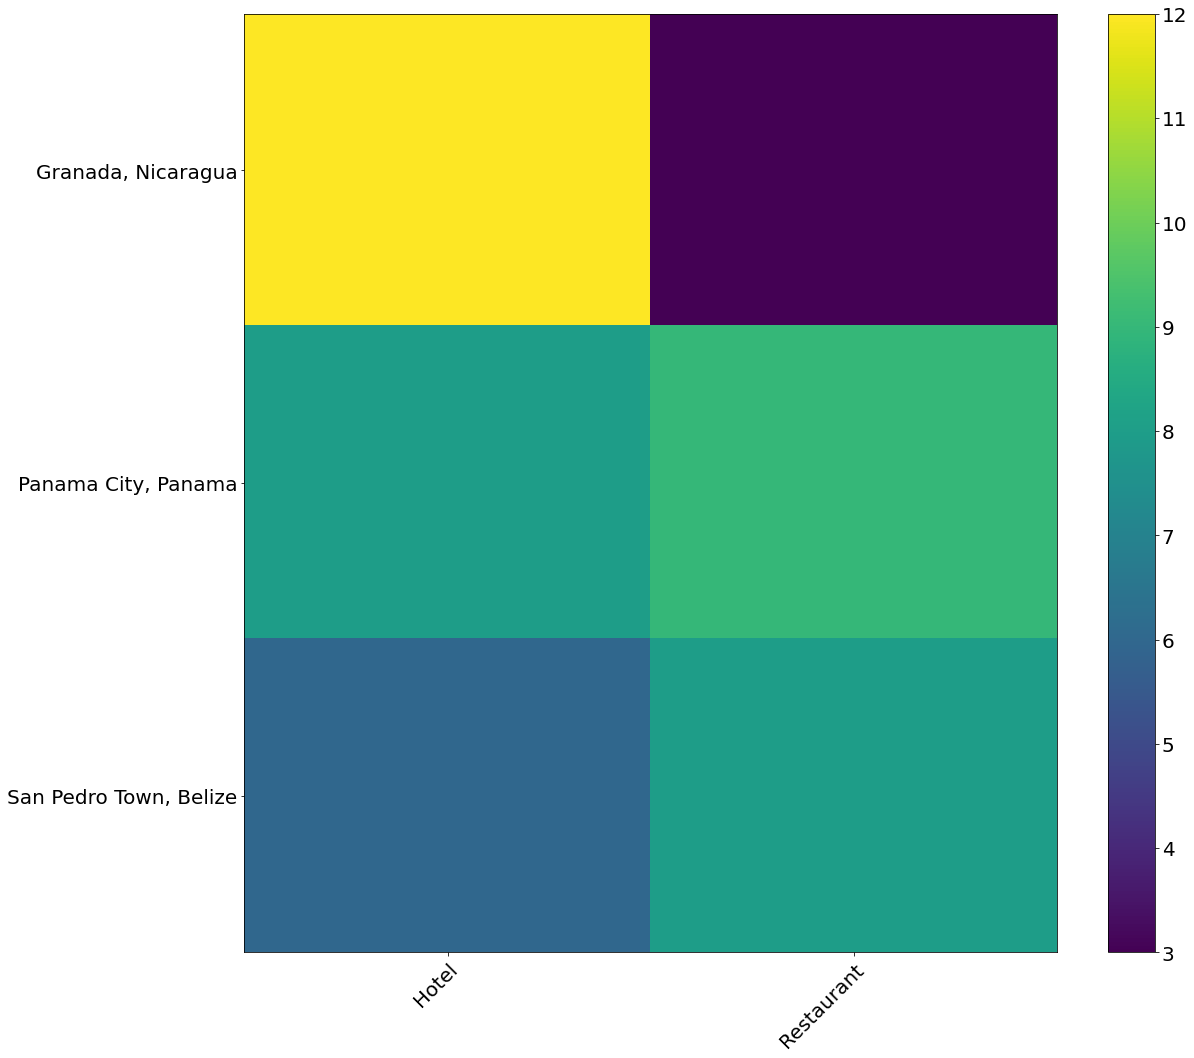
\includegraphics[width=\textwidth]{images/cluster6.png}
    \caption{Number of venues per category on the cities in the small cluster 3}
    \label{fig:cluster_5}
\end{figure}



\section{Discussion}

The small clusters are very special because they group cities with particular venues categories. Besides, they have many of the same types, so they might not be attractive to investors looking to grow some businesses in the region. Another one that doesn't look appealing is the few businesses groups. It has plenty of venue categories which makes it very difficult to identify consumption patterns or trends. The gathered information is not enough to find a market niche where a new company is needed in these cities. 


The most exciting clusters are the gastronomic and the busy group. They are related due to the similar venues categories that they gather, which are associated with food. Two opportunities for investment can be made: hotels and new spaces.

From the results, we can see that even though there are many activities regarding restaurants, there are not many hotels. So there is an opportunity to tap into the hospitality business and highlight those cities as gastronomical destinations that can be combined with the region's cultural heritage and natural resources. 

Knowing the consumption trends at these clusters shows where people like to go and the places they frequently visit. Creating new venues or spaces in the same category might be an excellent option to invest in. Always trying to separate the brand with unique and distinguishable characteristics. 

The recommendation is to start testing business initiatives in the cities of the gastronomic clusters due to the already identified business trends and because they have a relatively small number of venues.

\section{Conclusion}

The best cities to start a business are: Alajuela (Costa Rica), Belize City (Belize), Chinandega (Nicaragua), La Ceiba (Honduras), León (Nicaragua), Limón (Costa Rica), Masaya (Nicaragua), México (Guatemala), Puntarenas (Costa Rica), San Miguelito (Panamá) or Santa Ana (El Salvador). The category should be related to gastronomy or hospitality.

Taking advantage of machine learning techniques helps answer critical business questions and removes uncertainty, making better decisions.

Getting and combining different data sources can produce exciting results, primarily when nontraditional data sources like API are used.

Investigating business insights, consumption trends, and behavior patterns is a heavy duty that can be simplified through technological tools and provide positive results.  

\printbibliography

\pagebreak
\pagebreak
\section{Tables}

%\begin{table}[]
%\caption{Most important cities of Central America}
%\label{tab:my-table}
%\begin{tabular}{lll}
\begin{longtable}{c c c c }
\caption{Most important cities of Central America} \\
\label{tab:table1}
\textbf{City}                   & \textbf{Province}             & \textbf{Country}  \\
\hline\endhead
\hline \endfoot 
San José                 & San José             & Costa Rica  \\
Alajuela                 & Alajuela             & Costa Rica  \\
Cartago                  & Cartago              & Costa Rica  \\
Heredia                  & Heredia              & Costa Rica  \\
Puntarenas               & Puntarenas           & Costa Rica  \\
Limón                    & Limón                & Costa Rica  \\
Liberia                  & Guanacaste           & Costa Rica  \\
San Isidro de El General & San José             & Costa Rica  \\
Quesada                  & Alajuela             & Costa Rica  \\
Desamparados             & San José             & Costa Rica  \\
Managua                  & Managua              & Nicaragua   \\
León                     & León                 & Nicaragua   \\
Masaya                   & Masaya               & Nicaragua   \\
Matagalpa                & Matagalpa            & Nicaragua   \\
Tipitapa                 & Managua              & Nicaragua   \\
Chinandega               & Chinandega           & Nicaragua   \\
Jinotega                 & Jinotega             & Nicaragua   \\
Granada                  & Granada              & Nicaragua   \\
Estelí                   & Estelí               & Nicaragua   \\
Puerto Cabezas           & RACCN                & Nicaragua   \\
San Salvador             & San Salvador         & El Salvador \\
Santa Ana                & Santa Ana            & El Salvador \\
Soyapango                & San Salvador         & El Salvador \\
San Miguel               & San Miguel           & El Salvador \\
Santa Tecla              & La Libertad          & El Salvador \\
Mejicanos                & San Salvador         & El Salvador \\
Apopa                    & San Salvador         & El Salvador \\
Delgado                  & San Salvador         & El Salvador \\
Ahuachapán               & Ahuachapán           & El Salvador \\
Ilopango                 & San Salvador         & El Salvador \\
Tegucigalpa              & Francisco Morazán    & Honduras    \\
San Pedro Sula           & Cortés               & Honduras    \\
La Ceiba                 & Atlántida            & Honduras    \\
Choloma                  & Cortés               & Honduras    \\
El Progreso              & Yoro                 & Honduras    \\
Comayagua                & Comayagua            & Honduras    \\
Choluteca                & Choluteca            & Honduras    \\
Danlí                    & El Paraíso           & Honduras    \\
La Lima                  & Cortés               & Honduras    \\
Villanueva               & Cortés               & Honduras    \\
Guatemala City           & Guatemala            & Guatemala   \\
Mixco                    & Guatemala            & Guatemala   \\
Villa Nueva              & Guatemala            & Guatemala   \\
Cobán                    & Alta Verapaz         & Guatemala   \\
Quetzaltenango           & Quetzaltenango       & Guatemala   \\
Jalapa                   & Jalapa               & Guatemala   \\
Escuintla                & Escuintla            & Guatemala   \\
San Juan Sacatepéquez    & Guatemala            & Guatemala   \\
Jutiapa                  & Jutiapa              & Guatemala   \\
Petapa                   & Guatemala            & Guatemala   \\
Panama City              & Panamá               & Panama      \\
San Miguelito            & Panamá               & Panama      \\
Las Cumbres              & Panamá               & Panama      \\
La Chorrera              & Panamá Oeste         & Panama      \\
Tocumen                  & Panamá               & Panama      \\
Pacora                   & Panamá               & Panama      \\
Arraiján                 & Panamá Oeste         & Panama      \\
David                    & Chiriquí             & Panama      \\
Santiago de Veraguas     & Veraguas             & Panama      \\
Belize City              & Belize District      & Belize      \\
San Pedro Town           & Belize District      & Belize      \\
Dangriga                 & Stann Creek District & Belize      \\
Ladyville                & Belize District      & Belize     \\
\end{longtable}

\end{document}
